
\documentclass[9pt,a4paper,twoside]{tau}
% \usepackage[spanish,es-nodecimaldot,es-noindentfirst]{babel}
\usepackage[english]{babel}
\usepackage{graphicx}
\usepackage{tau}
\usepackage{float}
\usepackage{multicol}

%----------------------------------------------------------
% Title
%----------------------------------------------------------

\title{Custom CPU Architecture: ARM Cortex M0 implementation}

%----------------------------------------------------------
% Authors, affiliations and professor
%----------------------------------------------------------

\author[a]{David Ortiz Cota}
\author[a]{Sebastián Pulido Espinoza}
\author[a]{Alfredo Romo}
\author[a]{Jorge González Díaz}

%----------------------------------------------------------

\affil[a]{Student}
% \affil[b]{Affiliation of author two}
% \affil[c]{Affiliation of author three}

\professor{José Ignacio Parra Vilchis}

%----------------------------------------------------------
% Footpage notes
%----------------------------------------------------------

\institution{Tec de Monterrey, Campus Guadalajara}
\ftitle{}
\date{Jun 5, 2024}
\etal{}
\course{System on Chip Design}

%----------------------------------------------------------
% Abstract
%----------------------------------------------------------

\begin{abstract}    
    This paper delves into the intricate design and implementation of a complete microprocessor based on the ARM Cortex M0 Harvard architecture. Moving beyond a single instruction, it explores the fundamental building blocks that orchestrate the complex process of fetching, decoding, and executing instructions. The paper outlines the core architecture of the microprocessor, including the key functional units like the Control Unit, Arithmetic Logic Unit (ALU), Program Memory, register file and RAM. It delves into the instruction set architecture (ISA), detailing the instruction formats, addressing modes, and their impact on program execution. The implementation details encompass the logic design principles employed for each unit, exploring the data flow and control signals that govern their operation. Furthermore, the paper discusses the memory hierarchy and its interaction with the processor.\\
    Finally, the paper touches upon the challenges encountered during implementation, potential optimization strategies, and the verification methodologies used to ensure the microprocessor's functionality. This comprehensive exploration provides valuable insights into the intricate world of microprocessor design, serving as a valuable resource for computer architecture students and professionals.
\end{abstract}

%----------------------------------------------------------

\keywords{Arm Cortex M0, Harvard, Microcontroller, Microprocessor, Verilog, FPGA board, Hardware Description Language, Soft processor}

%----------------------------------------------------------

\begin{document}
	
    \maketitle
    \thispagestyle{firststyle}
    \abscontent
    \tableofcontents

%----------------------------------------------------------


%----------------------------------------------------------%
%%                   INTRODUCTION                         %%
%----------------------------------------------------------%
\section{Introduction}

    \taustart{M}icroprocessors, the brains of modern computing devices, orchestrate the complex dance of data processing that powers our digital world. This paper embarks on a journey to unravel the intricacies of microprocessor design and implementation, delving into the fundamental principles that govern these remarkable machines.

    A microprocessor is a computer processor for which the data processing logic and control is included on a single integrated circuit (IC), or a small number of ICs. The microprocessor contains the arithmetic, logic, and control circuitry required to perform the functions of a computer's central processing unit (CPU). The IC is capable of interpreting and executing program instructions and performing arithmetic operations. The microprocessor is a multipurpose, clock-driven, register-based, digital integrated circuit that accepts binary data as input, processes it according to instructions stored in its memory, and provides results (also in binary form) as output. Microprocessors contain both combinational logic and sequential digital logic, and operate on numbers and symbols represented in the binary number system.

    \subsection{Brief History of Microprocessors.}
    It all began with the invention of the transistor by Bell Labs in the 1950s. These tiny, solid-state devices replaced bulky and power-hungry vacuum tubes, paving the way for smaller and more efficient electronic circuits. This technological leap laid the foundation for the integrated circuit (IC), a revolutionary concept conceived by Jack Kilby at Texas Instruments (TI) in 1958. The IC miniaturized electronics even further by integrating multiple transistors onto a single silicon chip, dramatically reducing size and complexity. \\
    The year 1971 witnessed the birth of the first commercially available microcontrollers. There's some debate about which device holds this title. The Texas Instruments TMS 1000, developed by Gary Boone and Michael Cochran, is widely recognized as a pioneer. This 4-bit microcontroller had a simple instruction set, built-in memory, and rudimentary input/output (I/O) capabilities, making it suitable for basic control tasks. Around the same time, Intel released its 4-bit 4004. Initially designed for calculators, the 4004's versatility and low cost led to broader applications in control systems. These early microcontrollers marked the beginning of a new era in embedded computing.

    \subsection{Existing Architectures}
    There are 2 main existing architectures used nowadays, they are Von Neumann Architecture and Harvard Architecture.

        \subsubsection{Hardvard Architecture:}
        The Harvard architecture is a computer architecture with separate storage and signal pathways for instructions and data. It is often contrasted with the von Neumann architecture, where program instructions and data share the same memory and pathways. This architecture is often used in real-time processing or low-power applications.
        There is no need to make the two memories share characteristics. In particular, the word width, timing, implementation technology, and memory address structure can differ. In some systems, instructions for pre-programmed tasks can be stored in read-only memory while data memory generally requires read-write memory. In some systems, there is much more instruction memory than data memory so instruction addresses are wider than data addresses.
    
        \subsubsection{Von Neumann Architecture}
        The von Neumann architecture is a foundational design concept for computers. It features a unified memory space that stores both program instructions and data. The CPU fetches both from this single location, simplifying the overall design and control logic. This architecture typically involves sequential access, where instructions and data are retrieved one after another. While this can be efficient for applications where instruction and data access are balanced, it can create bottlenecks for tasks requiring frequent data manipulation, as the CPU might need to wait for data retrieval before continuing program execution. Despite this potential drawback, the von Neumann architecture remains popular due to its simplicity, ease of programming, and cost-effectiveness, making it a suitable choice for general-purpose computing.
    
    \subsection{Existing implementations}
    There also 2 main existing implementations, they are the Complex Instruction Set Computer (CISC) and Reduced Instruction Set Computer (RISC). An instruction set, also known as an Instruction Set Architecture (ISA), is essentially the language a processor understands. It defines a set of commands that the processor can execute to perform various operations. These operations can be simple, like adding two numbers, or more complex, like moving data between memory locations or controlling external devices.

        \subsubsection{RISC}
        RISC processors focus on a smaller set of simpler instructions. These instructions typically perform a single, well-defined operation. While they might require more instructions to achieve the same result as a single CISC instruction, their simplicity allows for faster execution and optimization. RISC processors often excel in performance due to their simpler instructions. These instructions can be decoded and executed more efficiently, leading to faster processing speeds.
        Well-known RISC architectures include ARM (used in most mobile devices) and SPARC (developed by Oracle).

        \subsubsection{CISC}
        CISC processors boast a rich set of complex instructions. These instructions can perform multiple operations in a single step, making programming potentially easier and more intuitive for developers. For example, a single CISC instruction might add two numbers and store the result in a specific memory location. While CISC instructions can be efficient for some tasks, their complexity can sometimes lead to slower execution compared to RISC. Decoding these complex instructions can take time, and they might not always be perfectly optimized for the hardware. Popular CISC architectures include the x86 family (used by Intel and AMD) and the POWER architecture (developed by IBM).

    
    
    

%----------------------------------------------------------%
%%                   Design & implementation              %%
%----------------------------------------------------------%
\section{Design and Implementation}
    Our architecture is based on an Arm Cortex M0 3-stage architecture.\\
    The 3-stage pipeline is a fundamental concept in computer architecture that optimizes the instruction processing speed within a CPU. It breaks down the instruction execution process into three distinct stages, allowing the CPU to work on multiple instructions simultaneously.\\
\subsection{Pipeline overview}
    \begin{itemize}
        \item 1. Fetch (Instruction Fetch):
        In this stage, the CPU fetches an instruction from memory based on the address provided by the program counter (PC). Think of it like a librarian retrieving a book (instruction) from the shelf (memory) based on the call number (PC).
        \item 2. Decode (Instruction Decode): Once fetched, the instruction is passed to the decode stage. Here, the control unit deciphers the instruction by analyzing its opcode (operation code) and operands.
        Imagine the librarian decoding the Dewey Decimal System (opcode) and identifying the section (data to be processed) and category (operation) of the book (instruction).
        \item 3. Execute (Instruction Execution): In the final stage, the decoded instruction is executed. The control unit sends control signals to the relevant ALU (Arithmetic Logic Unit) or other execution units based on the instruction type (addition, data transfer, etc.). The ALU performs the designated operation and stores the result. This stage is like the librarian following the instructions (data and operation) in the book (instruction) to perform a specific task (calculation, data movement).
    
    \end{itemize}
    

\begin{figure}[h]  % The [h] here is a placement specifier (here)
    \centering  % This command centers the image
    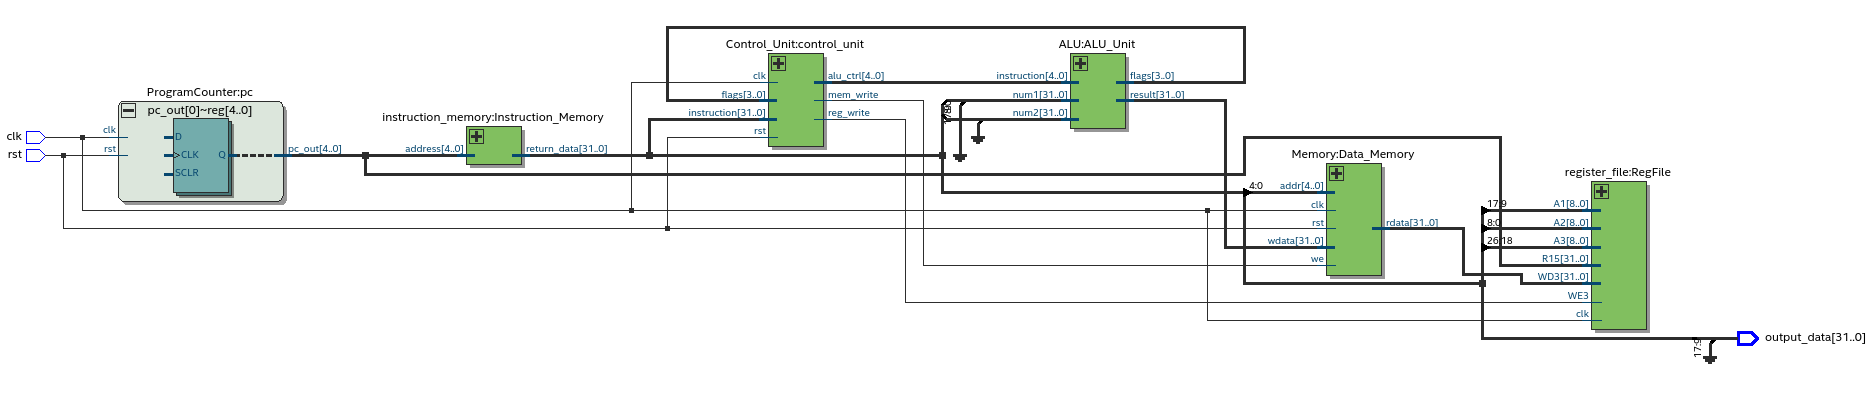
\includegraphics[width=0.5\textwidth]{images/RTLImg.png}
    \caption{RTL Overview}
    \label{fig:my_label}
\end{figure}

%----------------------------------------------------------%
%%                   
%%                      Modules
%%
%----------------------------------------------------------%




\subsection{Modules}
There are 5 main modules that form the CPU, the \textit{Program Counter}, \textit{Instruction Memory}, \textit{ALU}, \textit{Data Memory}, \textit{Register File}.\\ Each one of them will be explained in detail, as well as there individual inputs and outputs:

%----------------------------------------------------------%
%%                   PROGRAM COUNTER
%----------------------------------------------------------%
\subsubsection{PC}
    The program counter (PC), also known as instruction pointer (IP), is a critical register within the CPU of a microprocessor. It acts like a conductor's baton, keeping track of the memory address from which the next instruction will be fetched. In essence, the PC dictates the execution flow of a program by specifying the sequence of instructions to be processed by the CPU.

    The value of the program counter can be modified to allow for \textit{jumps} and \textit{branches} (which have yet to be implemented in our architecture). In our PC implementation, the program counter starts and resets at 0, and count up by 1 every clock cicle.\\
    
    \textbf{Inputs}:
    \begin{itemize}
        \item Clock and Reset: the value PC value increments by 1 every clock cicle and resets to 0 when the reset signal is enabled 
    \end{itemize}
    \textbf{Outputs}:
    \begin{itemize}
        \item PC Value: the actual value of the PC, will be the address of the instruction retrieved from the \textit{Instruction Memory}.
    \end{itemize}
    
    \begin{figure}[h]  % The [h] here is a placement specifier (here)
        \centering  % This command centers the image
        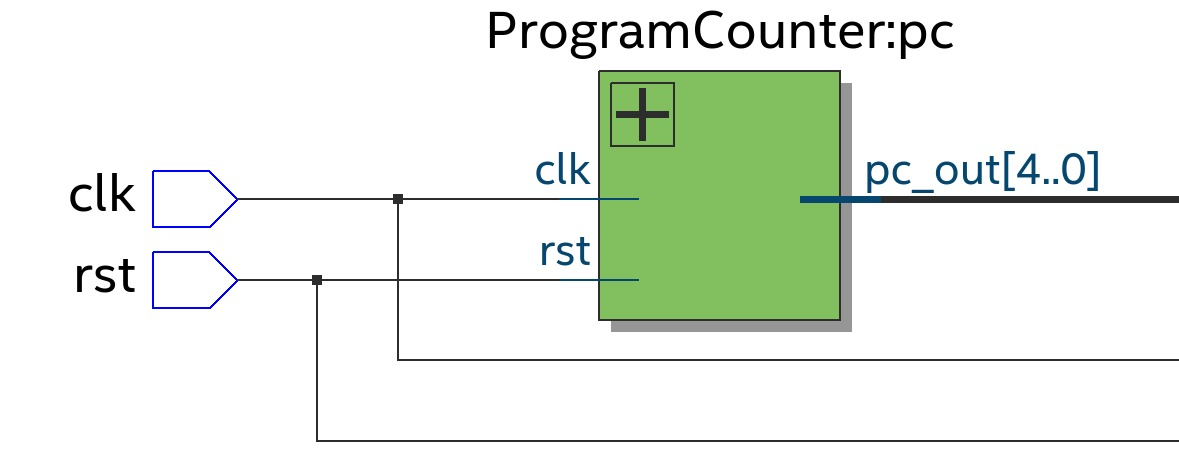
\includegraphics[width=0.3\textwidth]{images/PCImg.png}
        \caption{Program Counter RTL}
        \label{fig:my_label}
    \end{figure}





%----------------------------------------------------------%
%%                   INSTRUCTION MEMORY
%----------------------------------------------------------%
\subsubsection{Instruction Memory}
    The instruction memory module, often abbreviated as IM, serves as the brain's storage room for a program's instructions within a microprocessor. It's a read-only memory (ROM) specifically designed to hold the sequence of instructions that make up the software being executed. \\

    The main functions of the Instruction Memory are the following:

    \begin{itemize}
        \item \textbf{Storage}: The IM stores the program code in the form of binary machine code instructions. These instructions are pre-loaded before program execution and remain fixed throughout.
        \item \textbf{Retrieval}: When the program counter sends a memory address, the instruction memory acts like a lookup table. It retrieves the instruction located at that specific address.
        \item \textbf{Feeding the Pipeline}: The retrieved instruction is then fed into the processor's pipeline for decoding and execution. This fetch-decode-execute cycle continues until the program terminates.\\
    \end{itemize}

    \textbf{Inputs}:
    \begin{itemize}
        \item Address: Program counter output (interpreted as the address to retrieve from memory).

    \end{itemize}
    
    \textbf{Outputs}:
    \begin{itemize}
        \item Instruction: 32-bit instruction retrieved from memory.
    \end{itemize}


    \begin{figure}[h]  % The [h] here is a placement specifier (here)
        \centering  % This command centers the image
        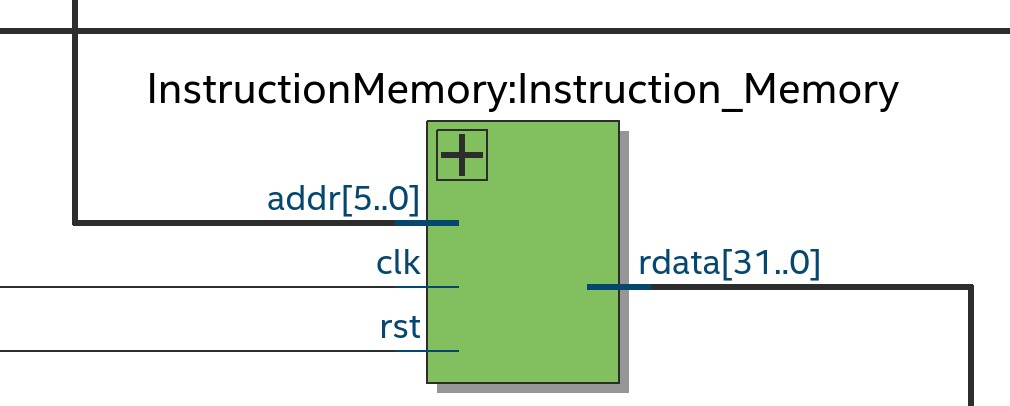
\includegraphics[width=0.5\textwidth]{images/InstMemImg.png}
        \caption{Instruction Memory RTL}
        \label{fig:my_label}
    \end{figure}
    
%----------------------------------------------------------%
%%                   CONTROL UNIT
%----------------------------------------------------------%
\subsubsection{Control Unit}
    The control unit (CU) acts as the conductor of the orchestra within a microprocessor's central processing unit (CPU). It's the central brain that interprets instructions, coordinates execution, and ensures all the other parts work together seamlessly. The details of its operation are the following:

    \begin{itemize}
        \item \textbf{Instruction Decoding}: Once fetched, the CU decodes the instruction to understand the operation it represents. This involves deciphering the binary code of the instruction and identifying what needs to be done, it takes the first 5 bits of the instruction and interprets it as an OPCODE, the remaining bits are interpreted as \textit{destination} for the selected operation (9-bits), and operands 1 \& 2 (9-bits and 9-bits).
        
        \item \textbf{Issuing Control Signals}: Based on the decoded instruction, the CU generates control signals that act like instructions for other CPU components. These signals direct the arithmetic logic unit (ALU) to perform calculations, tell registers where to store data, and coordinate communication with memory and input/output devices.
        
        \item \textbf{Execution Flow Management}: The CU doesn't just issue commands; it also manages the overall flow of program execution. It determines the sequence of steps involved in executing an instruction and ensures they happen in the correct order. This might involve fetching operands (data to be manipulated), sending them to the ALU, and then storing the results. \\ 

    \end{itemize}

    \textbf{Inputs}:
    \begin{itemize}
        \item Clk and Rst: Clock and reset signals.
        \item Instruction: 32-bit instruction received from Instruction  Memory.
        \item Flags: flags recieved from a previous ALU operation.
    \end{itemize}
    
    \textbf{Outputs}:
    \begin{itemize}
        \item Memory to Register: Enables whether the memory output should be written to registers.
        \item Memory Write Enable: Write enable signal for Data Memory
        \item Alu Control: 5 bit OPCODE for ALU in case the instruction requires it
    \end{itemize}
    


    \begin{figure}[h]  % The [h] here is a placement specifier (here)
        \centering  % This command centers the image
        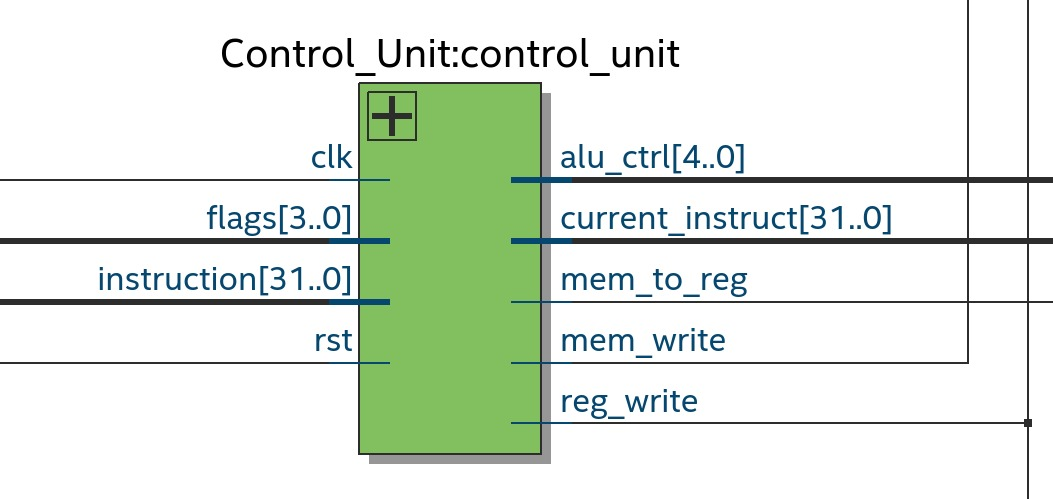
\includegraphics[width=0.3\textwidth]{images/CUImg.png}
        \caption{Control Unit RTL}
        \label{fig:my_label}
    \end{figure}



%----------------------------------------------------------%
%%                   ALU
%----------------------------------------------------------%
\subsubsection{ALU}
    The ALU, which stands for Arithmetic Logic Unit, is the workhorse of the CPU (Central Processing Unit)  when it comes to performing calculations and making logical decisions. It can do arithmetic operation like addition and subtraction, Logical operations like comparing 2 numbers, and bitwise operations like shifts

    \textbf{Inputs}:
    \begin{itemize}
        \item Instruction: 5-bit OPCODE that gets interpreted as a certain operation via a demultiplexer.
        \item Num1 \& Num2: Operands for operations
    \end{itemize}
    
    \textbf{Outputs}:
    \begin{itemize}
        \item Flags: Flags raised by certain operations. Our architecture includes flags for \textit{Negative, Zero, Carry \& oVerflow}
        \item Result: 32-bit result from whatever operation was performed by the Alu.
    \end{itemize}
    



    \begin{figure}[h]  % The [h] here is a placement specifier (here)
        \centering  % This command centers the image
        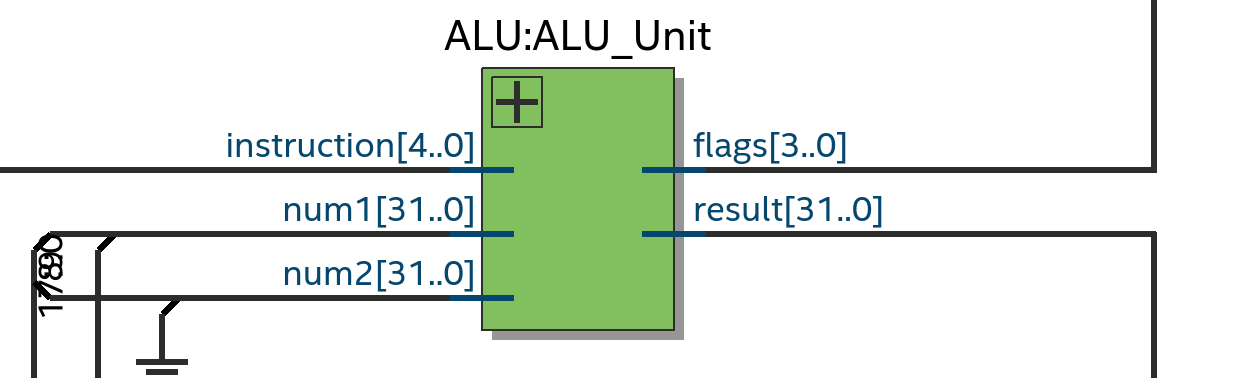
\includegraphics[width=0.5\textwidth]{images/ALUImg.png}
        \caption{ALU RTL}
        \label{fig:my_label}
    \end{figure}


%----------------------------------------------------------%
%%                   DATA MEMORY
%----------------------------------------------------------%
\subsubsection{Data Memory}
    Data memory, also commonly referred to as RAM (Random Access Memory), is the work area of a microprocessor where it stores and retrieves the temporary data that's actively used during program execution. Unlike instruction memory, which holds the program instructions permanently, data memory is constantly changing as the program progresses. It serves as the temporary storage space for various types of data, including:
    Variables, Intermediate Results, Function Arguments, Return Values and Heap Memory.\\
    Data memory is volatile, meaning it loses its content when the power is turned off. This is because RAM uses capacitors to store data, and these capacitors discharge over time without a constant power supply.\\

    \textbf{Inputs}:
    \begin{itemize}
        \item Clk and Rst: When the rst signal is active, the memory resets to all 0's.
        \item we: Write enable to determin read or write operation.
        \item wdata: Data to be written to a certain memory address (in case write enable is active).
        \item Address: Address to be writen or retrieved from memory.
    \end{itemize}
    
    \textbf{Outputs}:
    \begin{itemize}
        \item Return Data: If write enable is disabled, the data fetched will be returned via this bus.
    \end{itemize}


    \begin{figure}[h]  % The [h] here is a placement specifier (here)
        \centering  % This command centers the image
        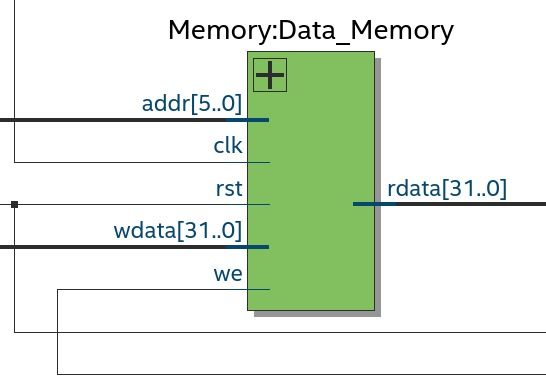
\includegraphics[width=0.3\textwidth]{images/DataMemImg.png}
        \caption{Data Memory RTL}
        \label{fig:my_label}
    \end{figure}
    






%----------------------------------------------------------%
%%                   REGISTER FILE
%----------------------------------------------------------%
\subsubsection{Register File}
    The register file is a set of high-speed internal memory locations within the CPU (Central Processing Unit).  They act as the CPU's scratchpad or workbench, holding frequently accessed data and intermediate results for quick manipulation. Compared to main memory (data memory), registers offer significantly faster access times, making them critical for efficient program execution. \\
    This implementation consist of a 14+1 register file. The first 14 registers act general function registers, while the 15th register gets its value from the program counter + 2, the purpose of this offset is to compensate for the 2 clock cicles that have elapsed (Fetch/Decode) from the previous clock cicles.

    \textbf{Inputs}:
    \begin{itemize}
        \item Clk and Rst: When the rst signal is active, the memory resets to all 0's.
        \item A1 \& A2: Addresses to be acted upon, received from the instruction.
        \item A3: Writeback address.
        \item WE3: Write enable from address 3 (recieved from the Control Unit).
        \item R15: Value recieved from the program counter (+2 for reasons mentioned above).
    \end{itemize}
    
    \textbf{Outputs}:
    \begin{itemize}
    \item RD1 \& RD2: Return data from A1 and A2, used as the operands for the ALU.
    \end{itemize}
    


    \begin{figure}[h]  % The [h] here is a placement specifier (here)
        \centering  % This command centers the image
        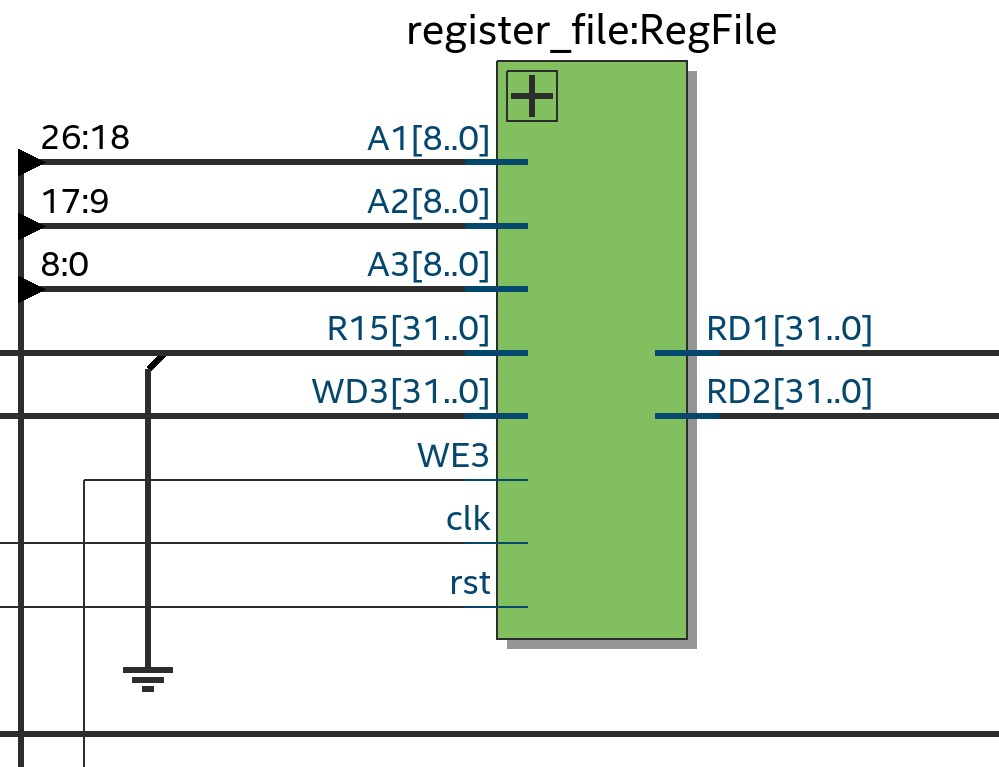
\includegraphics[width=0.27\textwidth]{images/RegFileImg.png}
        \caption{Register File RTL}
        \label{fig:my_label}
    \end{figure}



\section{Case of Study:}


     
\section{Conclusion}
\justifying

    This paper explored the design considerations and implementation details for a LOAD instruction within a custom architecture. We discussed the fundamental functionalities of the memory hierarchy, including instruction memory, data memory, registers, and the program counter. We then delved into the concept of the LOAD instruction, explaining its role in data transfer between memory and registers.\\
    
    The design of the LOAD instruction for a custom architecture requires careful consideration of factors such as:
    
    \begin{itemize}
        \item Instruction format: Defining the opcode, operand types (immediate, register addressing, memory addressing modes), and their encoding scheme.
        \item Memory access mechanisms: Specifying how the CPU calculates the effective memory address based on the chosen addressing mode.
        \item Interaction with other components: Ensuring proper coordination between the control unit, ALU, and data memory during the LOAD instruction execution.
        \item Pipeline compatibility: Designing the LOAD instruction to work seamlessly within the pipelined execution scheme of the processor, considering potential data hazards.
        \item By understanding these aspects and tailoring the design to the specific architecture requirements, we can create an efficient LOAD instruction that facilitates data movement and enables effective program execution. This paves the way for further development of the custom instruction set architecture (ISA) and the creation of a powerful and versatile processing unit.
    \end{itemize}


%----------------------------------------------------------

\addcontentsline{toc}{section}{References}
\printbibliography

%----------------------------------------------------------

\end{document}

%---------------- Exmaple note and code -------------------
\begin{info}	
        Lorem ipsum dolor sit amet, consectetur adipiscing elit. Sed vestibulum justo quis massa aliquet, ut ultrices quam bibendum.
\end{info}